\section{Lösungsansatz}

%----------------------------------------------------------------------%SLIDE -
\begin{frame}
    \frametitle{Lösungsansatz}

    \begin{itemize}
        \item Beschränkung auf $9 \times 9$ Bretter
        \item Feedforward Netze (TODO: Layout)
        \item Genetische Algorithmen (TODO: Parameter)
    \end{itemize}
\end{frame}
%----------------------------------------------------------------------%SLIDE -

%----------------------------------------------------------------------%SLIDE -
\begin{frame}
    \frametitle{Lösungsansatz}

    \begin{algorithm}[H]
        \caption{sequentielle Lösung}
        \begin{algorithmic}[1]
            \State $N_0 \gets \{ n$ zufällig generierte neuronale Netzwerke $\}$
            \For {$net \in N_0$}
                \State trainiere $net$ auf regelgerechtes Spielen
            \EndFor
            \For {Runde $i = 0$ bis $\ldots$}
                \For {$\forall net_a \neq net_b \in N_i$}
                    \State lass $net_a, net_b$ gegeneinander spielen
                    \State zähle die Anzahl der Siege
                \EndFor
                \State generiere $N_{i+1}$ mittels genetischen Algorithmus
                abhängig von $N_i$ und den Spielergebnissen
            \EndFor
            \State Speichere $N_n$
        \end{algorithmic}
    \end{algorithm}
\end{frame}
%----------------------------------------------------------------------%SLIDE -

%----------------------------------------------------------------------%SLIDE -
\begin{frame}
    \frametitle{UML}

    \begin{figure}
        \centering
        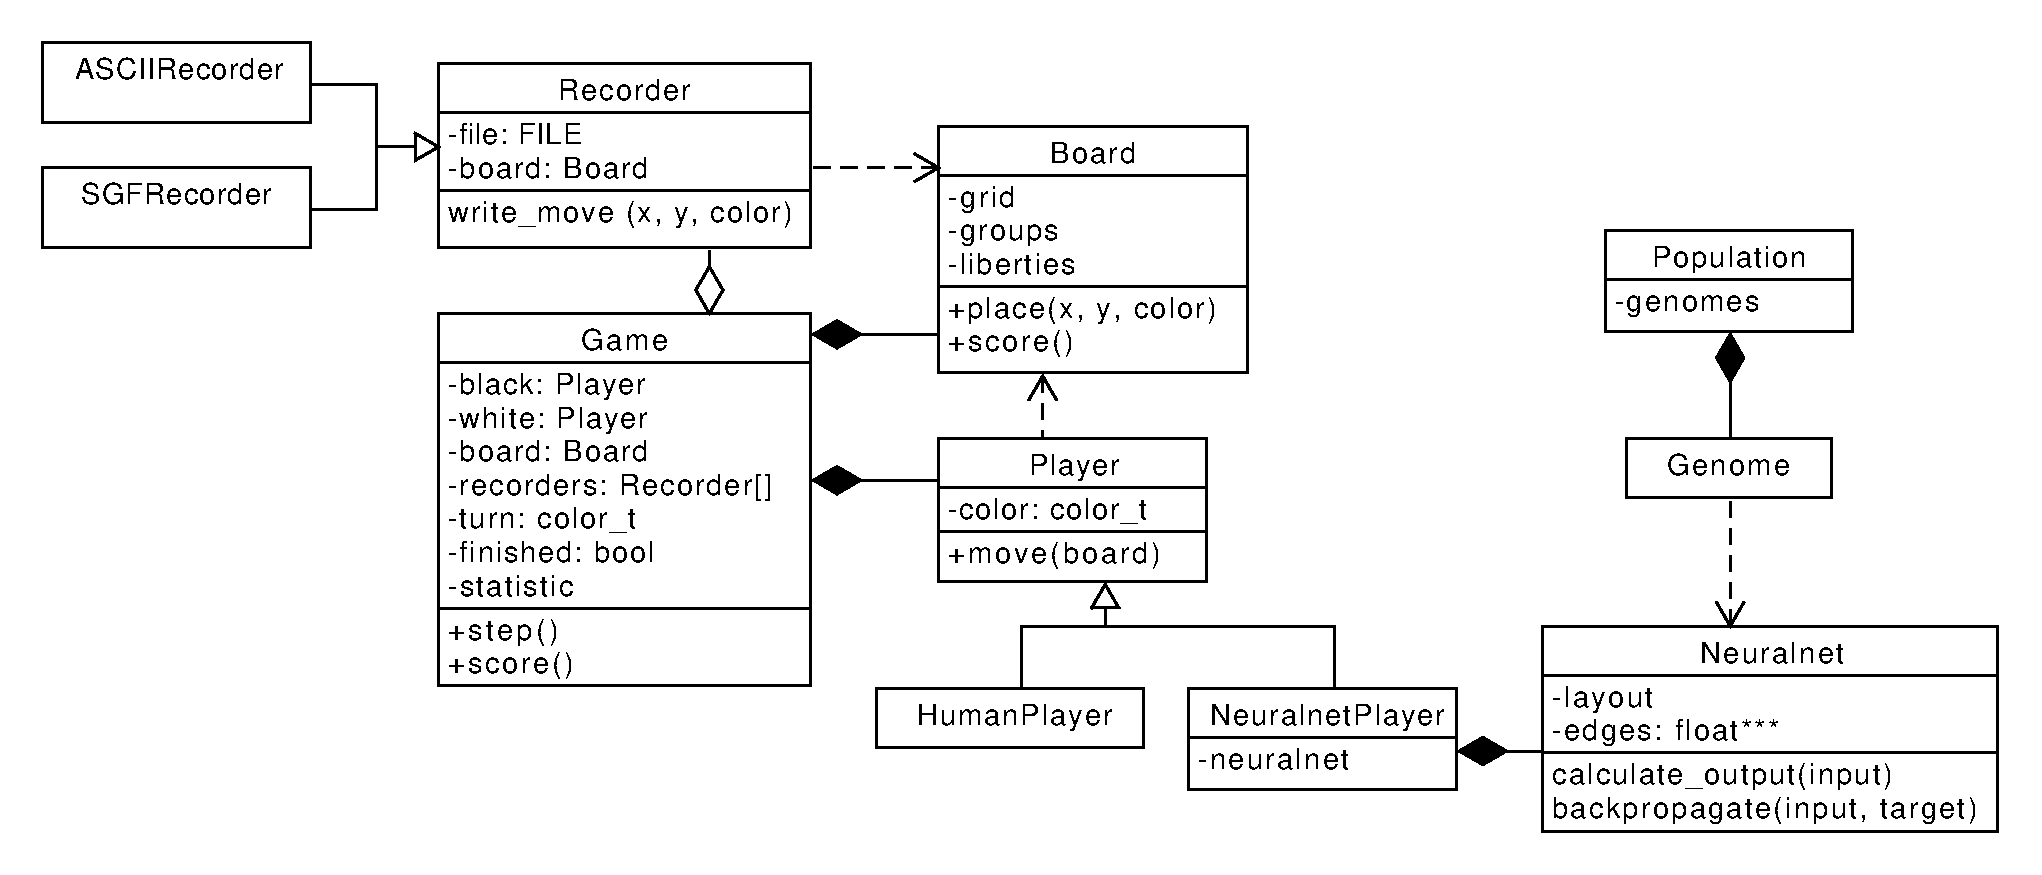
\includegraphics[scale=0.4]{content/img/class_diagram.pdf}
        \caption{Klassendiagramm}
    \end{figure}
\end{frame}
%----------------------------------------------------------------------%SLIDE -
